\documentclass[12pt,letterpaper]{article}
%\usepackage[utf8]{inputenc}
\UseRawInputEncoding
\usepackage[english]{babel}
\usepackage{listings}
\usepackage{xcolor}
\usepackage{graphicx}

%For syntax highlighting
\definecolor{codegreen}{rgb}{0,0.6,0}
\definecolor{codegray}{rgb}{0.5,0.5,0.5}
\definecolor{codepurple}{rgb}{0.58,0,0.82}
\definecolor{backcolour}{rgb}{1,1,1}

%%Sets different parameters
\lstdefinestyle{mystyle}{
    backgroundcolor=\color{backcolour},   
    commentstyle=\color{codegreen},
    keywordstyle=\color{magenta},
    numberstyle=\tiny\color{codegray},
    stringstyle=\color{codepurple},
    basicstyle=\ttfamily\footnotesize,
    breakatwhitespace=false,         
    breaklines=true,                 
    captionpos=b,                    
    keepspaces=true,                 
    numbers=left,                    
    numbersep=5pt,                  
    showspaces=false,                
    showstringspaces=false,
    showtabs=false,                  
    tabsize=4
}
\lstset{style=mystyle}

\title{\textbf{Department of Computer Science and Engineering}}
\author{\textbf{Shivanirudh S G, 185001146, Semester VII }}

\date{26 July 2021}

\begin{document}
\maketitle
\hrule
\section*{\center{UCS1711 - Mobile Application Development Lab}}
\hrule 
\bigskip\bigskip

%Assignment name
\subsection*{\center{\textbf{Exercise 2: Layouts and Event Listeners}}}

%Objective
\subsection*{\flushleft{Aim:}}
\begin{flushleft}
    Generate an application to simulate a calculator   
\end{flushleft}

%Code
\subsection*{\flushleft{Code:}}
\subsubsection*{\flushleft{Main Activity:}}
\textbf{Design:}
\begin{flushleft}
\lstinputlisting[language = XML]{Calculator/app/src/main/res/layout/activity_main.xml}
\end{flushleft}
\textbf{Behaviour:}
\begin{flushleft}
\lstinputlisting[language = JAVA]{Calculator/app/src/main/java/com/example/calculator/MainActivity.java}
\end{flushleft}

\newpage
\subsection*{\flushleft{Output:}}
\begin{figure}[h]
    \centering
    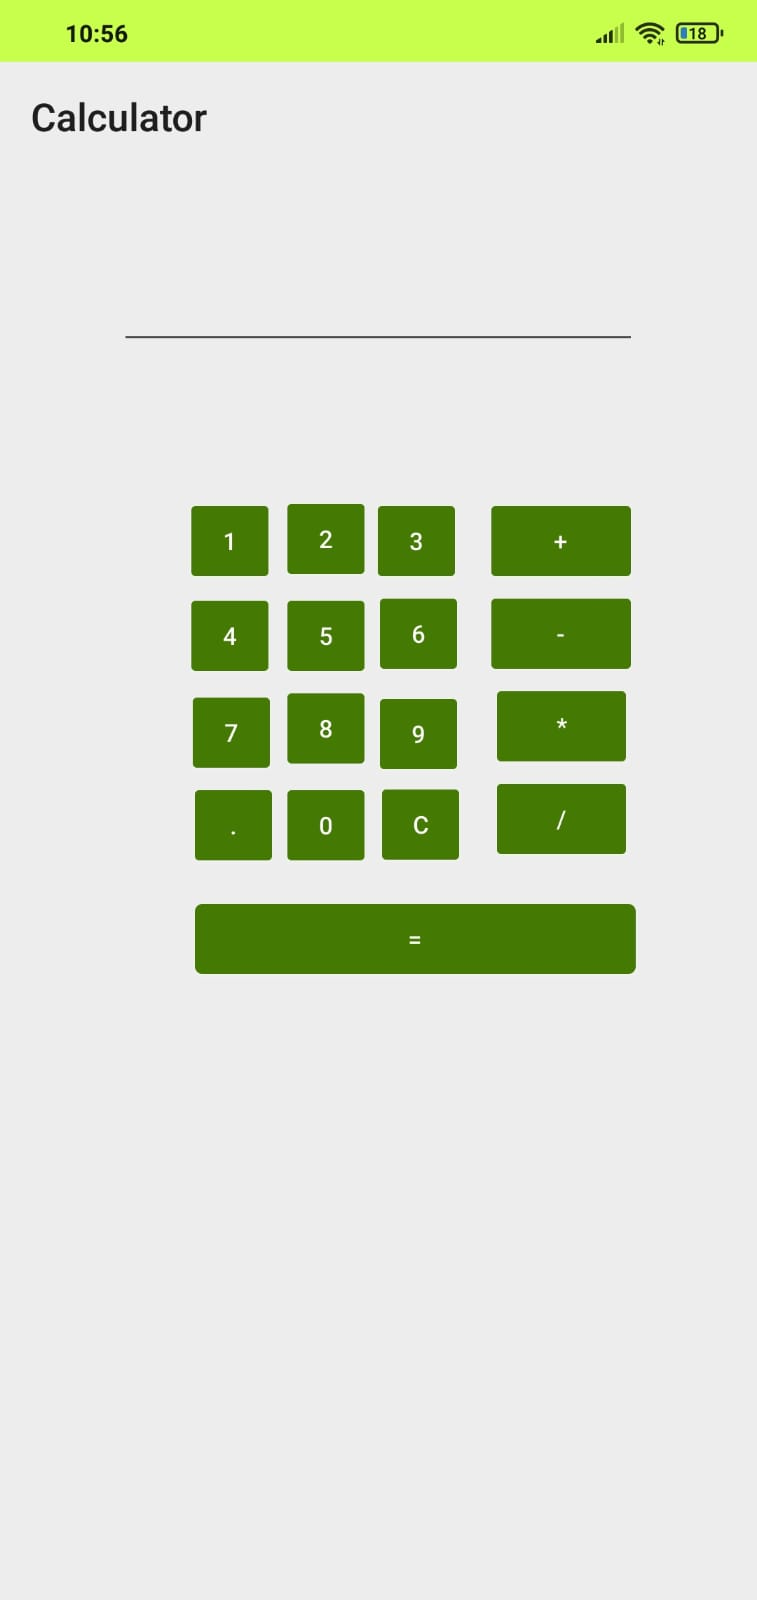
\includegraphics[height=14cm, keepaspectratio]{Calculator/Outputs/OP1.png}
\end{figure}
\begin{figure}
    \centering
    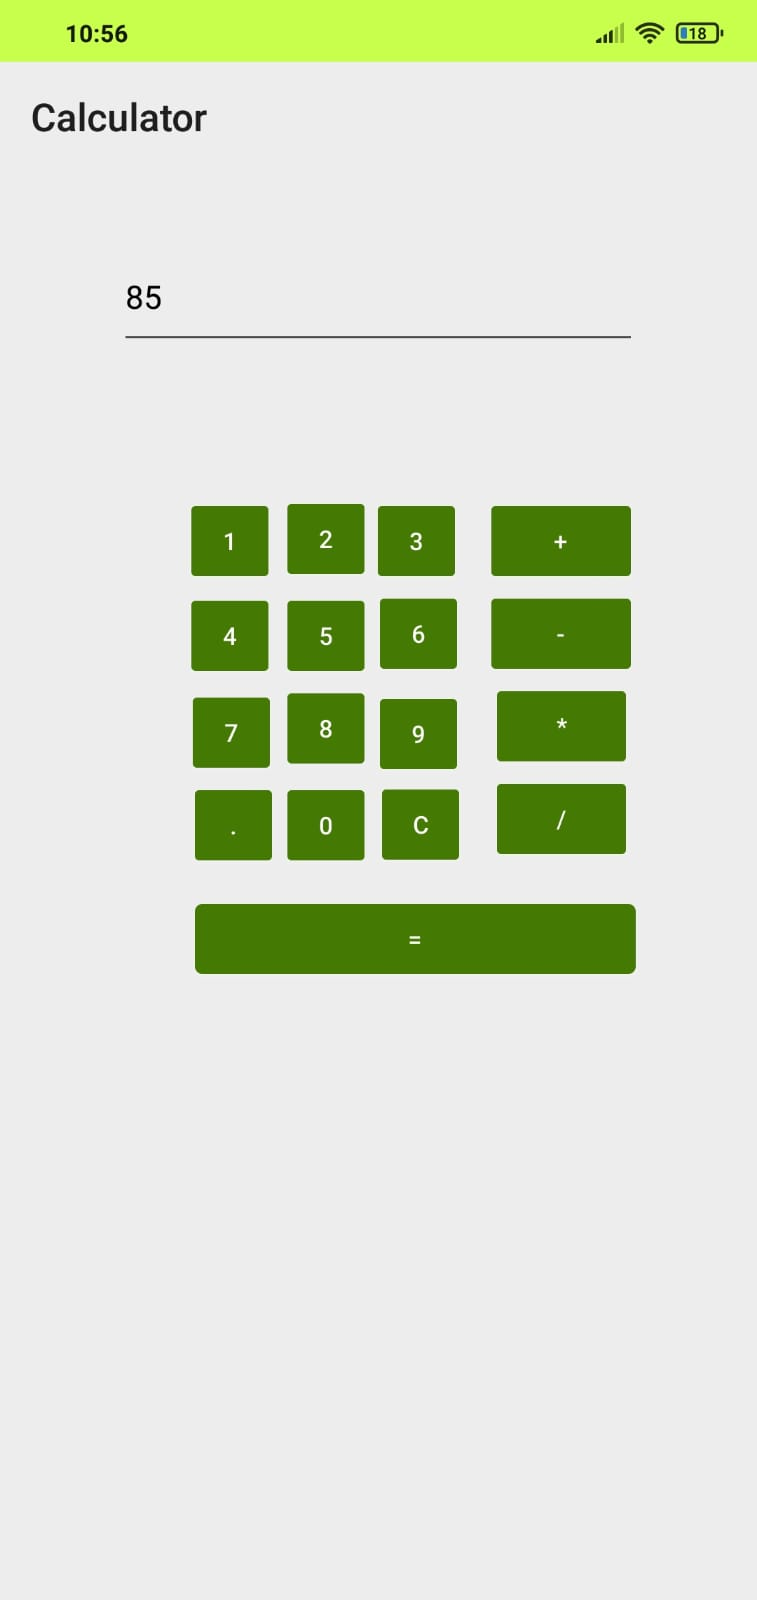
\includegraphics[height=14cm, keepaspectratio]{Calculator/Outputs/OP2.png}
\end{figure}
\begin{figure}
    \centering
    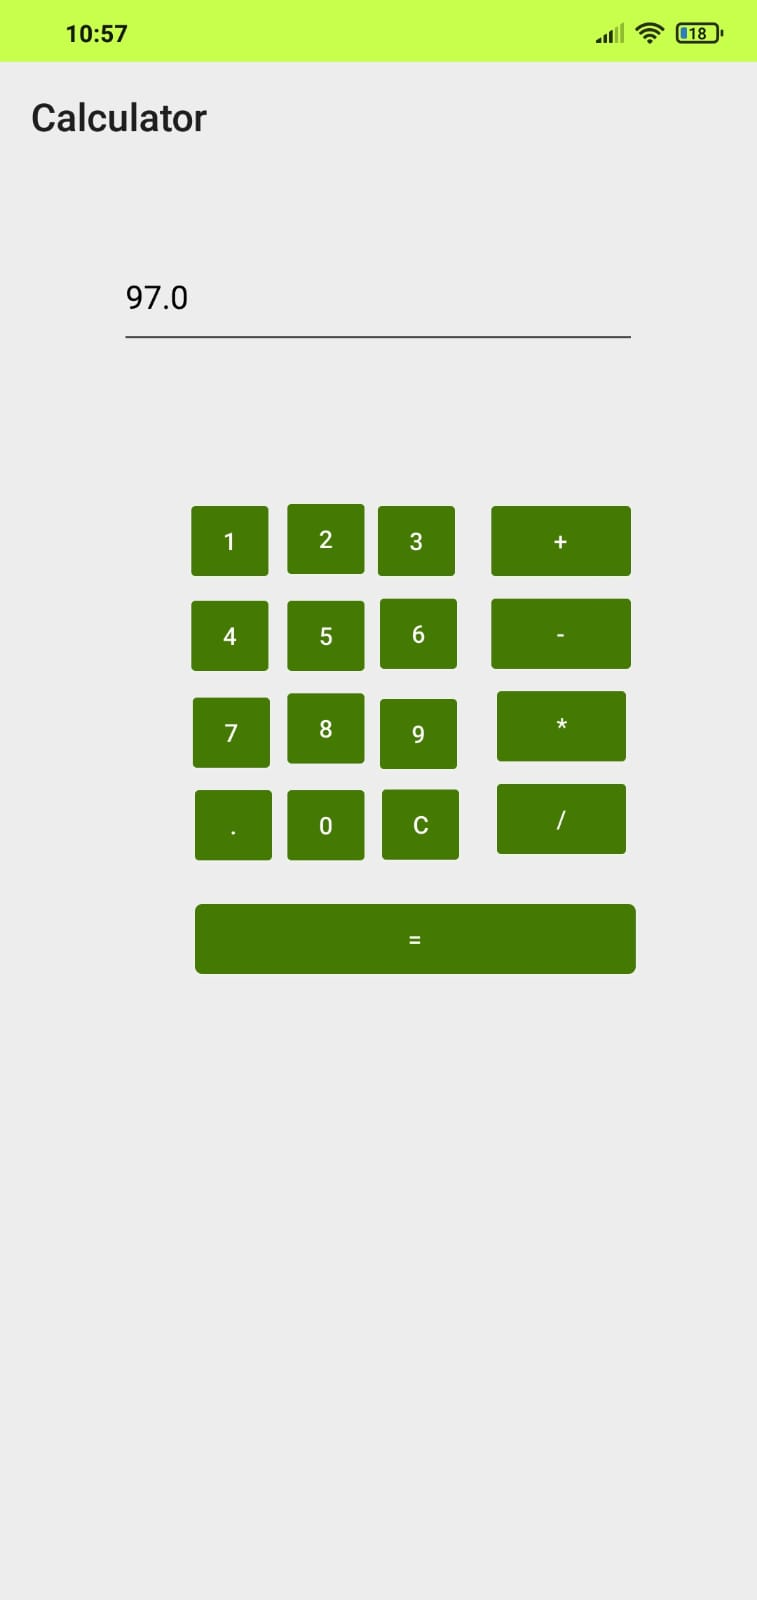
\includegraphics[height=14cm, keepaspectratio]{Calculator/Outputs/OP3.png}
\end{figure}

\newpage

\subsection*{\flushleft{Aim:}}
\begin{flushleft}
    Generate an application to simulate a keyboard  
\end{flushleft}

%Code
\subsection*{\flushleft{Code:}}

\subsubsection*{\flushleft{Keyboard Layout:}}
\textbf{Design:}
\begin{flushleft}
\lstinputlisting[language = XML]{Keyboard/app/src/main/res/layout/keyboard.xml}
\end{flushleft}
\textbf{Behaviour:}
\begin{flushleft}
\lstinputlisting[language = JAVA]{Keyboard/app/src/main/java/com/example/keyboard/CustomKeyboard.java}
\end{flushleft}

\subsubsection*{\flushleft{Main Activity:}}
\textbf{Design:}
\begin{flushleft}
\lstinputlisting[language = XML, lastline=32]{Keyboard/app/src/main/res/layout/activity_main.xml}
\end{flushleft}
\textbf{Behaviour:}
\begin{flushleft}
\lstinputlisting[language = JAVA]{Keyboard/app/src/main/java/com/example/keyboard/MainActivity.java}
\end{flushleft}

\newpage
\subsection*{\flushleft{Output:}}
\begin{figure}[h]
    \centering
    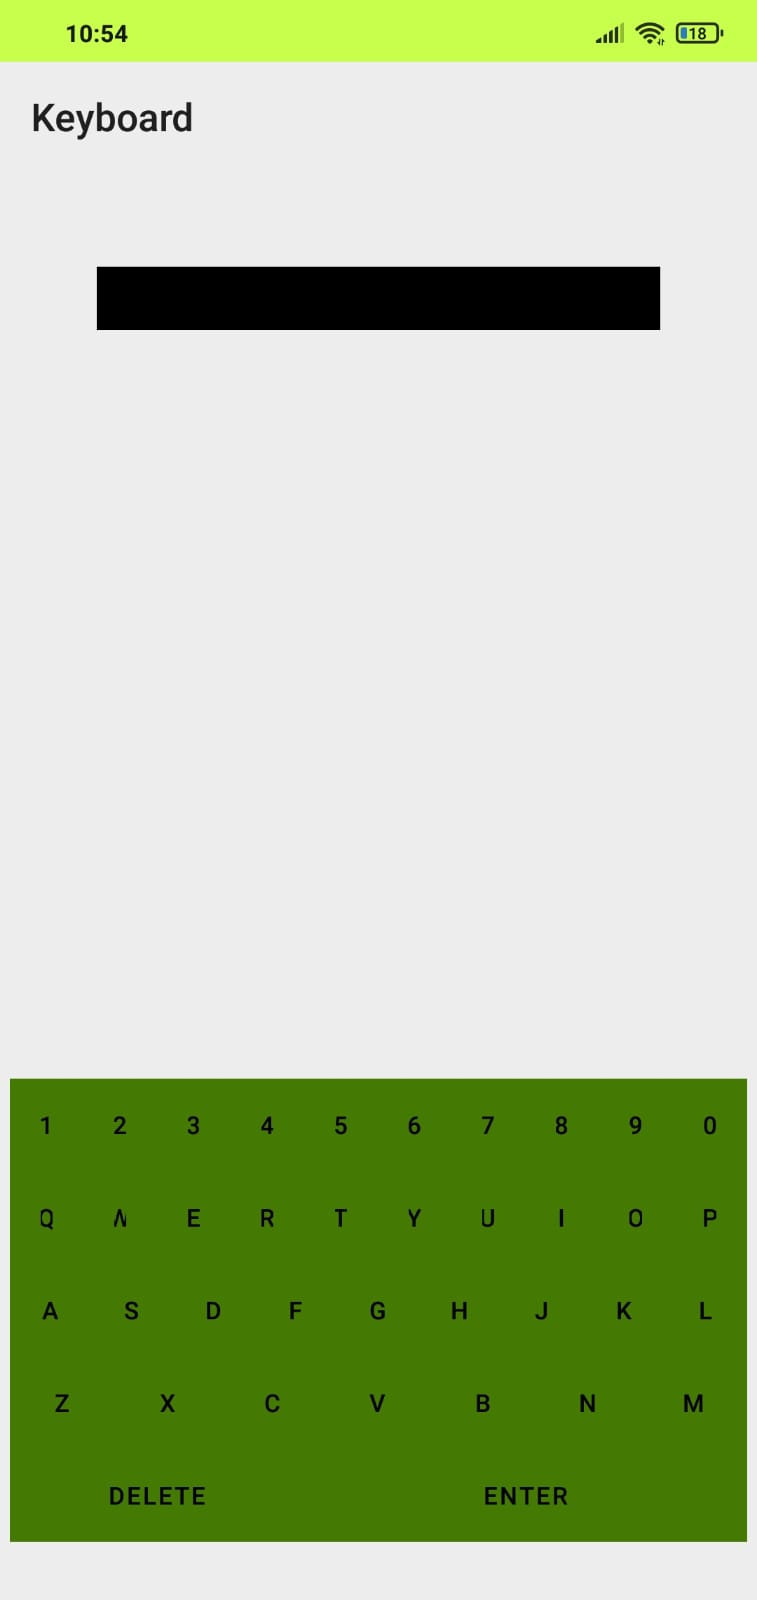
\includegraphics[height=14cm, keepaspectratio]{Keyboard/Outputs/OP4.png}
\end{figure}
\begin{figure}
    \centering
    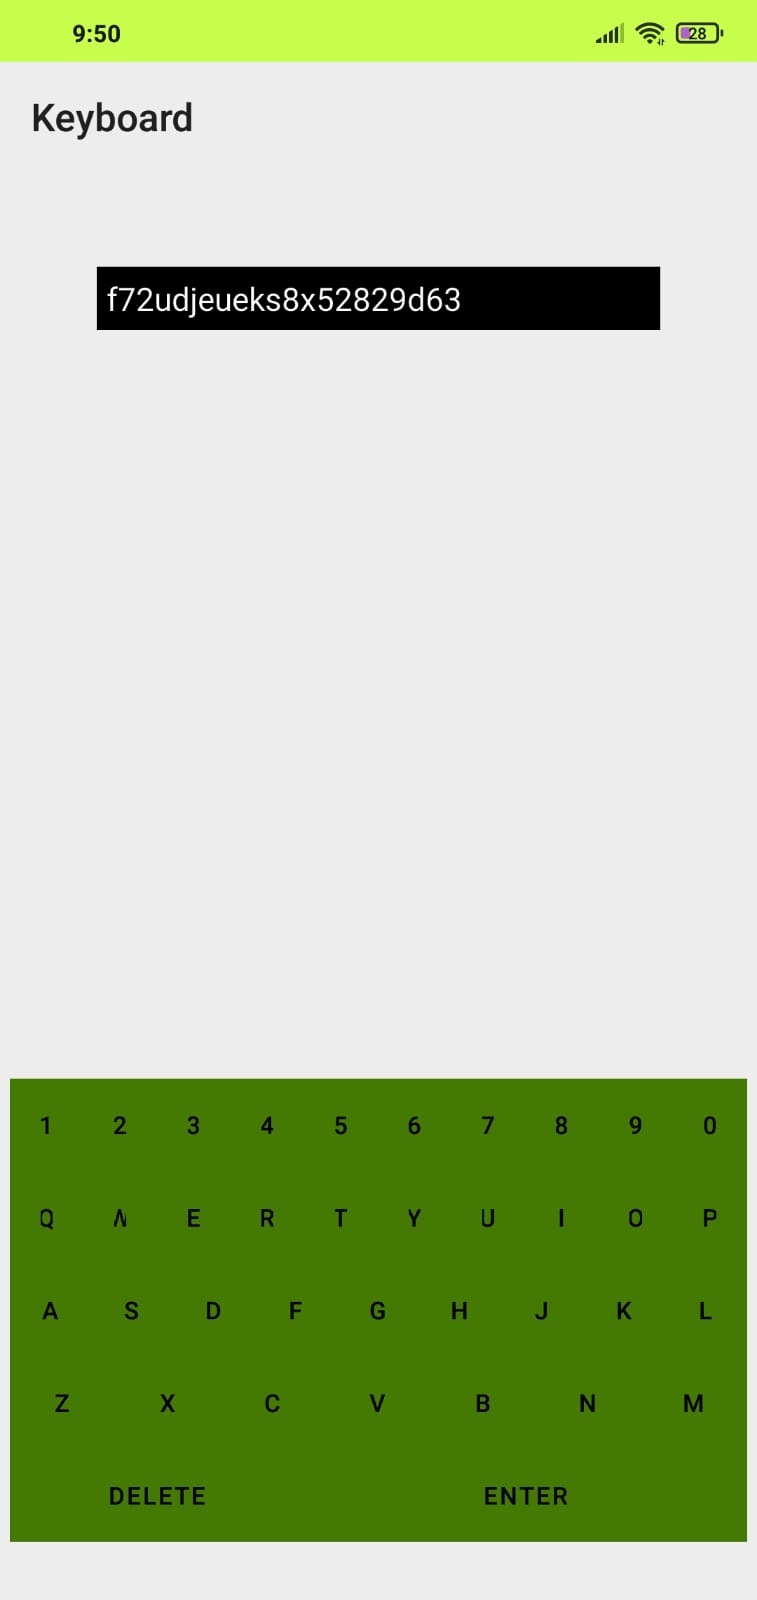
\includegraphics[height=14cm, keepaspectratio]{Keyboard/Outputs/OP1.png}
\end{figure}
\begin{figure}
    \centering
    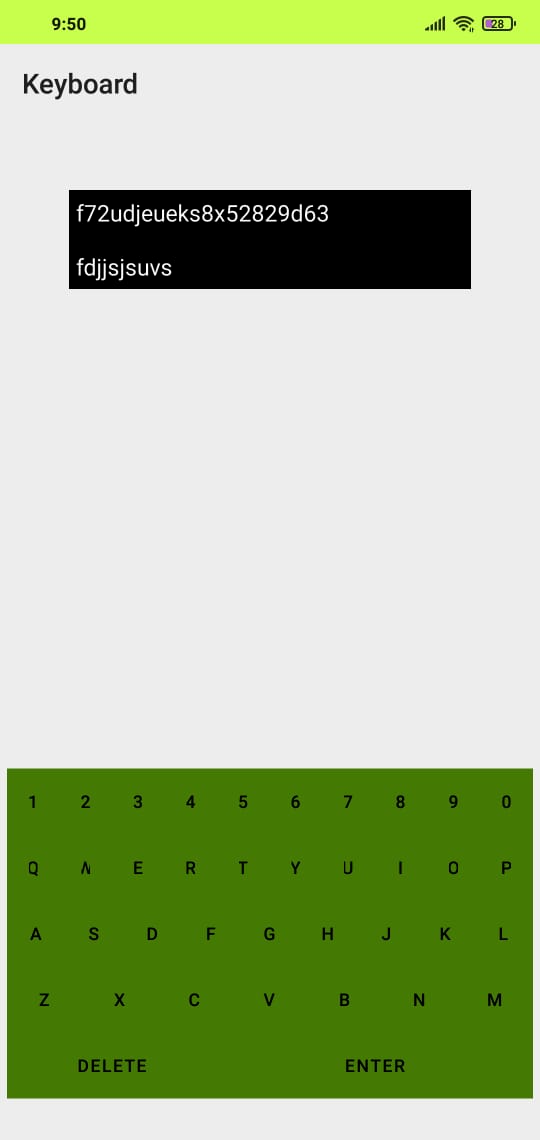
\includegraphics[height=14cm, keepaspectratio]{Keyboard/Outputs/OP2.png}
\end{figure}
\begin{figure}
    \centering
    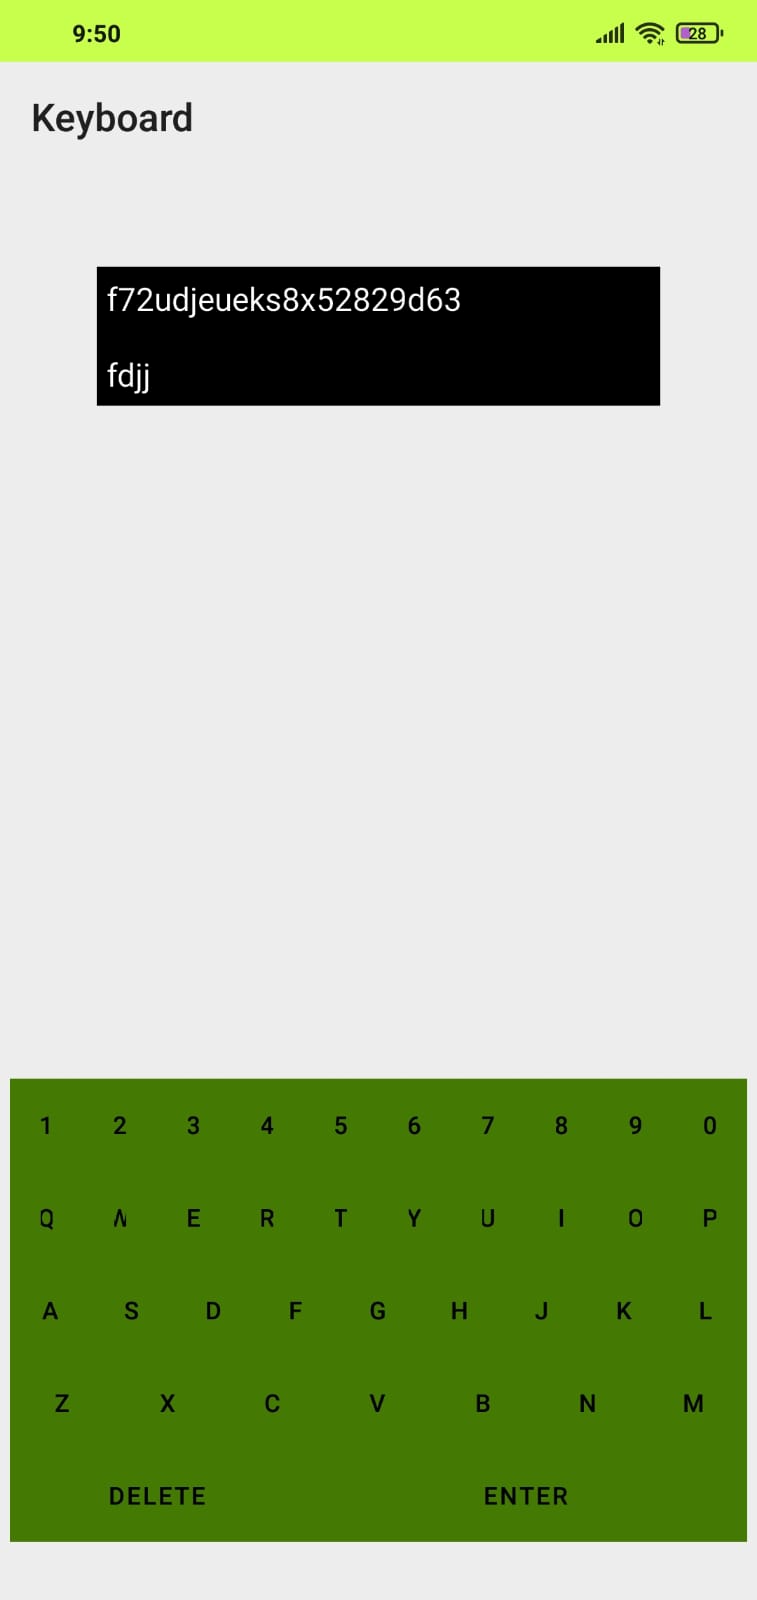
\includegraphics[height=14cm, keepaspectratio]{Keyboard/Outputs/OP3.png}
\end{figure}

\end{document}